\documentclass[11pt]{article} % Document type
\usepackage{graphicx}
\usepackage{float}
\usepackage{geometry}
\geometry{legalpaper, margin=1in}
\title{Assignment 3}
\author{Michael Kamensky}
\date{\today} % Sets the date to \today, or any date you specify
\begin{document}\maketitle % Start the document
\section{Running sorting}
Here is an example of runnig my tests:

\begin{verbatim}
mkamensk@vera:~/cse13s/asgn3$ ./sorting -a -n 15
Quick Sort, 15 elements, 135 moves, 51 compares
     34732749     42067670     54998264    102476060    104268822
    134750049    182960600    538219612    629948093    783585680
    954916333    966879077    989854347    994582085   1072766566

Shell Sort, 15 elements, 174 moves, 171 compares
     34732749     42067670     54998264    102476060    104268822
    134750049    182960600    538219612    629948093    783585680
    954916333    966879077    989854347    994582085   1072766566

Heap Sort, 15 elements, 144 moves, 70 compares
     34732749     42067670     54998264    102476060    104268822
    134750049    182960600    538219612    629948093    783585680
    954916333    966879077    989854347    994582085   1072766566

Batcher Sort, 15 elements, 90 moves, 59 compares
     34732749     42067670     54998264    102476060    104268822
    134750049    182960600    538219612    629948093    783585680
    954916333    966879077    989854347    994582085   1072766566
\end{verbatim}
\section{Moves}
This graph shows the amount Moves preformed by each algorithm compared to the number of elements
\begin{figure}[H]
\begin{center}
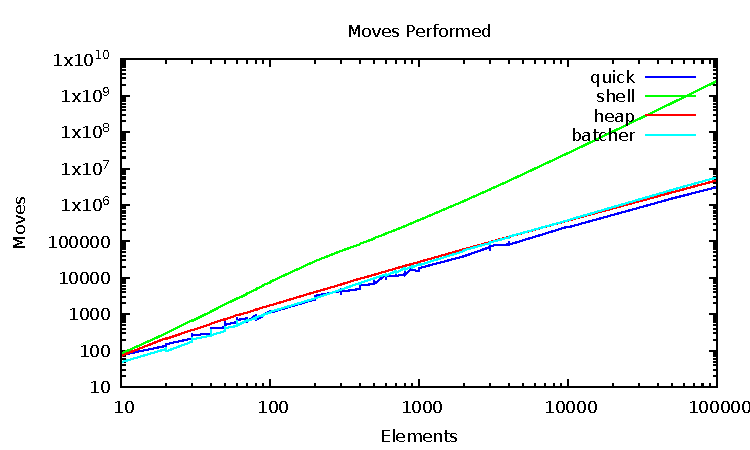
\includegraphics[height=3in,width=5in]{sorting.pdf}
\caption{graph produced by gnuplot with a different set of sorts for reference axes are log-scaled}
\end{center}
\end{figure}

\section{Compares}
This graph shows the amount of Compares preformed by each algorithm compared to the number of elements
\begin{figure}[H]
\begin{center}
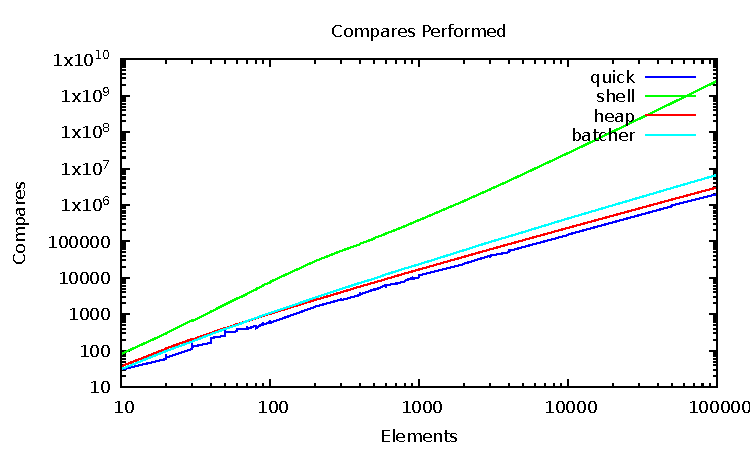
\includegraphics[height=3in,width=5in]{sorting_comp.pdf}
\caption{graph produced by gnuplot with a different set of sorts for reference axes are log-scaled}
\end{center}
\end{figure}

\section{Analysis}
As can be seen by the graphs Batcher sort works best when the list size is smaller it has the least amout of moves and compares.
Meanwhile quick sort seems to be better overall especially with larger list sizes it has less compares and moves then any other algorithm.
Shell sort is the worst overall with the highest number of compares and moves then any other algorithm. 
Finally, heap sort takes the middle of the pack it has niether the most or least amount of any compares of any sorting algorithm.
Addional note, my shell sort was different to the example sort due to the fact different gaps.h files where used; my gaps.h maximum gap size was set to defult 1000000.
Finally, the graph seems jagged because in my input data for each element size I have a several values for random seeds and therefore generate different random arrays.
I wanted to do that, to see how the number of moves and compares depends on input randomness.
Suprisingly it does not jump up and down very much, which means randomness does not play a large part in the algorithms efficiency, number of elements is determing factor.
\end{document}
